\documentclass[11pt]{article}
\usepackage[T1]{fontenc}
\usepackage{lmodern}
\usepackage[a4paper,margin=25mm,headheight=15pt]{geometry}
\usepackage{microtype,mathtools,amssymb,amsthm,booktabs,array,longtable,enumitem}
\usepackage{graphicx,xcolor,fancyhdr,needspace}
\definecolor{ink}{HTML}{16354A}
\definecolor{accent}{HTML}{167C80}
\usepackage[colorlinks=true,linkcolor=ink,citecolor=accent,urlcolor=accent]{hyperref}
\usepackage[nameinlink,noabbrev]{cleveref}
\hypersetup{pdftitle={A 5 by 5 Obstruction to Polynomial Ordered Matrix Removal},pdfauthor={Research draft for the ProveIt project}}
\pagestyle{fancy}\fancyhf{}
\fancyhead[L]{\small\textsc{Ordered matrix removal}}
\fancyhead[R]{\small Exact repair and sampling laws}
\fancyfoot[C]{\thepage}
\setlength{\parskip}{3pt}
\setlength{\parindent}{1.2em}
\setlist{itemsep=3pt,topsep=5pt}
\newtheorem{theorem}{Theorem}[section]
\newtheorem{lemma}[theorem]{Lemma}
\newtheorem{proposition}[theorem]{Proposition}
\newtheorem{corollary}[theorem]{Corollary}
\theoremstyle{definition}
\newtheorem{definition}[theorem]{Definition}
\newtheorem{question}[theorem]{Question}
\newtheorem{remark}[theorem]{Remark}
\newcommand{\one}{\mathbf 1}
\newcommand{\eps}{\varepsilon}
\newcommand{\E}{\mathbb E}
\newcommand{\Prob}{\mathbb P}
\newcommand{\dist}{\operatorname{dist}}
\newcommand{\Poi}{\operatorname{Poisson}}
\newcommand{\Cov}{\operatorname{Cov}}
\newcommand{\var}{\operatorname{Var}}
\newcommand{\Rset}{\mathsf R}
\newcommand{\Cset}{\mathsf C}
\newcommand{\crown}{\mathcal C}
\newcommand{\dd}{\mathrm d}
\newcommand{\fall}[2]{(#1)_{#2}}
\title{\color{ink}\textbf{A \(5\times5\) Obstruction to Polynomial\\Ordered Matrix Removal}\\[7pt]
\large Exact repair distance, copy packing, Poisson sampling,\\and an inverse logarithmic barrier}
\author{Research draft for the ProveIt project}
\date{7 October 2026}
\begin{document}
\maketitle
\begin{abstract}
The ordered binary matrix-removal construction in OpenAI's September 2026
manuscript uses a fixed \(66\times66\) forbidden matrix. We prove that its
anchor can be replaced by the three-by-three crown \(J_3-I_3\), giving an
explicit \(5\times5\) obstruction. The main structural tool is a
full-pattern pinning theorem: the body rows and columns resolve ambiguities
that the smaller anchor alone cannot resolve. The theorem uses nested
nonanchor traces, bounded anchor signatures, and a common mode order.
For the resulting matrices \(A_h\), with
\(m=2^h\) and \(n=(20h+2)m\), we determine three quantities exactly:
the number of forbidden copies is \(2m^8\), the minimum number of cells
meeting all existing copies is \(m\), and the minimum number of binary
entry changes producing a forbidden-pattern-free matrix is \(m^2\).
An explicit optimal repair changes one dummy-by-leaf rectangle; a
separate structural argument proves that this repair creates no new copies.

For independent uniform samples of \(q\) rows and \(q\) columns, the sharp
scale is \(q=(20h+2)m^{2/3}\). At a limiting multiple \(c\) of this scale,
the number of critical witnesses converges to \(\Poi(2c^3)\), and the
detection probability tends to \(1-e^{-2c^3}\). We also determine the
optimal order, and a variational leading constant, for entry queries using
uniform rectangular samples. Exact Lambert \(W\) inversion converts the
copy-transversal density into repair distance and gives a convergent
all-orders expansion of the resulting inverse logarithmic barrier.
A general bounded-signature theorem yields analogous constructions on
regular trees of every branching number. All proofs are included;
exhaustive finite checks and reproducible numerical illustrations accompany
the article.
\end{abstract}
\vspace{4pt}
\noindent\textbf{Keywords.} Ordered matrix removal; induced submatrices;
property testing; pinning; copy transversals; Poisson limits; Lambert \(W\).
\newpage
\begingroup\small
\tableofcontents
\endgroup
\newpage

\section{Problem, provenance, and main results}
\label{sec:intro}

An ordered copy of a binary \(k\times k\) matrix \(H\) in a binary
\(n\times n\) matrix \(A\) is a pair of strictly increasing maps
\(r,c:[k]\to[n]\) such that \(A(r(i),c(j))=H(i,j)\) for every \(i,j\).
Both zeros and ones are prescribed. Write \(N_H(A)\) for the number of
these copies, with no quotient by a symmetry factor, and put
\begin{equation}
 \dist_H(A)=\frac{1}{n^2}\min_{B:\,N_H(B)=0}
       |\{(x,y):A(x,y)\ne B(x,y)\}|.
 \label{eq:distance-definition}
\end{equation}
Changes from zero to one and from one to zero are both permitted.

The polynomial ordered binary matrix-removal question asks whether, for
every fixed \(H\), constants \(c_H,C_H>0\) satisfy
\begin{equation}
 \dist_H(A)\ge\eps
 \quad\Longrightarrow\quad
 N_H(A)\ge c_H\eps^{C_H}n^{2k}.
 \label{eq:polynomial-question}
\end{equation}
The finite-family form appears as Problem 1.4 of
Alon--Ben-Eliezer~\cite{AB2020}; the singleton form is Conjecture 4.5
of the first arXiv version of Gishboliner--Shapira~\cite{GS2025}.
Qualitative removal, without polynomial dependence, follows from
Alon--Ben-Eliezer--Fischer~\cite{ABF2017}. A related positive theorem says
that a polynomial density of \emph{entry-disjoint existing copies}
forces a polynomial total copy density~\cite[Theorem 1.2]{AB2020}.
The difference between a transversal of existing copies and a successful
binary repair is therefore central.

\subsection{The source construction and the new contribution}

OpenAI's manuscript \emph{Polynomial removal fails for ordered binary
matrices}, dated 25 September 2026, constructs a fixed \(66\times66\)
counterexample to \eqref{eq:polynomial-question}~\cite{OAI190}.
Its host is built from two signed copies of a binary tree, dummy positions,
and mode-specific anchors. The distance argument propagates incompatible
root bits to a shared leaf. Its large anchor identifies the mode of every
copy by combining density and a shattering block.

We retain that tree construction and propagation mechanism, with full
attribution, and replace the anchoring argument. A three-by-three crown
suffices when its two body rows and columns are included in the pinning
argument. The proof uses the absence of a nonanchor three-by-three crown,
nested traces within variable classes, at most two anchor signatures per
class, and the same mode order on both axes. The crown alone need not be
pinned. The full-pattern argument also survives an explicit optimal repair.
The resulting exact description of all copies then supports sharper
counting and sampling results.

The research selection also considered the asymptotic-reversion
work in ProveIt~\cite{ProveIt}. The present subject
has a finite combinatorial core suitable for independent checks, while
the exact hitting-to-repair conversion produces a direct application of
Lambert-centered asymptotic inversion. The proofs below depend on the
explicit matrix definitions, rather than on any unverified broad claim
elsewhere in either repository.

\begin{table}[ht]
\centering\small
\begin{tabular}{p{.27\textwidth}p{.30\textwidth}p{.32\textwidth}}
\toprule
Feature & OpenAI source~\cite{OAI190} & This article\\
\midrule
Forbidden pattern & \(66\times66\) & Explicit \(5\times5\)\\
Anchor & Dense \(64\times64\) matrix with shattering block & \(J_3-I_3\); full-pattern pinning\\
Host size & \((386h+2)2^h\) & \((20h+2)2^h\)\\
Repair distance & Lower bound from propagation & Exact value and optimal repair\\
Original-copy structure & Every copy meets a leaf diagonal & Complete classification and exact count\\
Balanced sample size & Necessary scale proportional to \(\sqrt m\) & Sharp scale proportional to \(m^{2/3}\)\\
Additional conclusions & Nonpolynomial removal & Exact packing; Poisson clustering; rectangular optimum; inverse expansion\\
\bottomrule
\end{tabular}
\caption{Comparison of the statements established in the specified source
with the refinements proved here. Host-size factors accompany the sampling
scales. The table does not assert a global minimal forbidden-pattern size.}
\label{tab:comparison}
\end{table}

\subsection{An explicit obstruction}

Let \(J_s\) denote the all-ones matrix and write \(\crown_s=J_s-I_s\).
Our forbidden matrix is
\begin{equation}
 H=\begin{pmatrix}
 0&1&1&1&0\\
 1&0&1&0&1\\
 1&1&0&0&0\\
 1&0&0&1&0\\
 0&1&0&1&1
 \end{pmatrix}
 =\begin{pmatrix}
 \crown_3&e_1&e_2\\ e_1^{\mathsf T}&1&0\\
 e_2^{\mathsf T}&1&1
 \end{pmatrix},
 \qquad P=\begin{pmatrix}1&0\\1&1\end{pmatrix}.
 \label{eq:H}
\end{equation}
Here \(e_1,e_2\) are the first two coordinate vectors of length three.

\begin{theorem}[Exact obstruction]
\label{thm:main}
For every integer \(h\ge1\), let
\[
 m=2^h,\qquad d=d_h=20h+2,\qquad n=dm,\qquad \eps_h=d^{-2}.
\]
There is an explicitly specified binary \(n\times n\) matrix \(A_h\) with
\begin{equation}
 N_H(A_h)=2m^8,\qquad
 \dist_H(A_h)=\eps_h.
 \label{eq:exact-main}
\end{equation}
The minimum number of cells meeting every existing \(H\)-copy is exactly
\(m\). There are \(m\) copies whose row sets are mutually disjoint and
whose column sets are mutually disjoint. In particular the maximum number
of entry-disjoint copies is also \(m\). Nevertheless, every successful
binary repair changes at least \(m^2\) entries, and a repair with exactly
\(m^2\) changes is given explicitly.
\end{theorem}

Thus the normalized copy density is exactly
\begin{equation}
 \delta_h:=\frac{N_H(A_h)}{n^{10}}
 =2d^{-10}m^{-2}=2\eps_h^5 4^{-h}.
 \label{eq:delta}
\end{equation}
For each fixed \(C>0\), \(\delta_h/\eps_h^C\to0\). This proves
failure of polynomial ordered removal for the particular matrix \eqref{eq:H}.
The smaller pattern is the main extremal refinement; the inverse-square
depth dependence of the distance remains that of the source mechanism.

\begin{theorem}[Balanced sampling law]
\label{thm:main-sampling}
Independently choose a uniform \(q_h\)-element row set and a uniform
\(q_h\)-element column set of \(A_h\), and let \(D_h\) be the event that
their intersection contains \(H\). If
\[
 \frac{q_h}{d_hm^{2/3}}\longrightarrow c\in(0,\infty),
\]
then a natural count \(X_h\) of leaf witnesses satisfies
\begin{equation}
 X_h\xrightarrow{\dd}\Poi(2c^3),\qquad
 \Prob(D_h)\longrightarrow1-e^{-2c^3}.
 \label{eq:main-poisson}
\end{equation}
Below this scale detection tends to zero; above it detection tends to one.
For fixed \(0<\rho<1\), the least balanced sample size with detection
probability at least \(\rho\) is
\begin{equation}
 q_{\rho,h}=d_hm^{2/3}
 \left(\frac{-\log(1-\rho)}{2}\right)^{1/3}(1+o(1)).
 \label{eq:quantile}
\end{equation}
\end{theorem}

This theorem concerns uniform row and column samples of equal size.
\Cref{sec:rectangles} treats unequal sizes and shows that allowing them
changes the optimal number of entry queries. The distinction is part of
the theorem's mathematical scope.

\subsection{Reading guide and verification status}

\Cref{sec:pinning} proves the general structural lemma;
\cref{sec:construction,sec:structure} define the host and verify every
hypothesis, including after repair. Exact copies and exact distance are
proved in \cref{sec:copies,sec:distance}. Sampling, inverse asymptotics,
and general branching are treated subsequently. The proofs are ordinary
mathematical proofs. The accompanying Python program checks finite
instances exactly; it is not a Lean formalization of the general theorems.
The source versions, contribution boundary, and proposed formalization
steps are recorded in \cref{sec:verification}.

\section{A pinning theorem from bounded signatures}
\label{sec:pinning}

For a row, its \emph{trace} on a collection of columns is its binary
restriction to those columns; column traces are defined in the same way.
Traces are \emph{nested} if their sets of ones are linearly ordered by
inclusion. This definition does not require the inclusion order to agree
with the ambient order of positions.

\begin{theorem}[Full-pattern pinning from bounded signatures]
\label{thm:pinning}
Let \(s\ge3\), let \(P\in\{0,1\}^{2\times2}\) satisfy \(P_{11}=1\),
and set
\begin{equation}
 K_s(P)=\begin{pmatrix}
 \crown_s&e_1&e_2\\
 e_1^{\mathsf T}&P_{11}&P_{12}\\
 e_2^{\mathsf T}&P_{21}&P_{22}
 \end{pmatrix},
 \label{eq:general-pattern}
\end{equation}
where the coordinate vectors have length \(s\). Consider an ordered
binary matrix with an anchor prefix on each axis, partitioned into
modes and then into \(s\) consecutive groups in the order
\(1,\ldots,s\). The modes must occur in the same order on both axes.
Assume the following properties on both axes.
\begin{enumerate}[label=\textnormal{(\roman*)}]
\item Within a mode the anchor blocks are the blow-up of \(\crown_s\);
between different modes their entries are zero. Positions in the same
anchor group have identical full traces.
\item The nonanchor positions are partitioned into variable classes and
an optional dummy class. Members of a dummy class have identical full
traces.
\item The nonanchor one-neighborhood of any anchor position is empty or
is contained in one class of the partition in (ii).
\item Against the anchor groups of a fixed mode, a nonanchor position has
ones in at most one group.
\item Within each variable class, traces on all opposite nonanchor
positions are nested, and traces on all opposite anchor positions take
at most \(s-1\) distinct values.
\item The nonanchor submatrix contains no \(\crown_3\), even under
separate permutations of three selected rows and columns.
\end{enumerate}
Then the first \(s\) rows and columns of every ordered \(K_s(P)\)-copy
use exactly one position from each anchor group of a single mode.
The last two positions on each axis are nonanchors, with the prescribed
\(e_1,e_2\) signatures against that mode's anchor.
\end{theorem}

\begin{proof}
Let \(r,c\in\{0,\ldots,s\}\) count the anchor positions among the
first \(s\) selected rows and columns. They are prefix counts because
every anchor precedes every nonanchor. The leading \(\crown_s\) has
distinct row traces and distinct column traces, so (i) forbids repeating
an anchor group among those rows or columns.

First suppose \(r,c\ge2\). Let \(t_1\le t_2\) be the modes of
the first two selected rows and \(u_1\le u_2\) those of the first
two selected columns, using the common mode order. The entries at
\((1,2)\) and \((2,1)\) are one, so (i) gives
\(t_1=u_2\) and \(t_2=u_1\). Therefore
\[
 t_1\le t_2=u_1\le u_2=t_1,
\]
and all four modes coincide, say with \(t\). If \(c<s\), the first
nonanchor column in the prefix has index \(c+1\ge3\), so it is one
against both first anchor rows. Their groups are distinct, contradicting
(iv). Hence \(c=s\), and the same argument on the other axis gives
\(r=s\). Every remaining leading row and column has a positive entry
against one of the first two opposite groups, which forces it into mode
\(t\). Distinctness and order then give every group of \(t\) exactly once.

Next suppose \(r,c\le1\). If \(r=c=0\), the leading prefix contains
the nonanchor \(\crown_3\) excluded by (vi). If \(r=1\), the last
two prefix columns are nonanchors and are both one against the first
anchor row. By (iii) they belong to one class. A dummy class would give
identical full column traces; a variable class would give nested traces
on nonanchor rows. Both contradict the \(\crown_2\) at the intersection
of the last two prefix rows and columns, all of which are nonanchors.
The case \(r=0,c=1\) follows by the same argument with axes exchanged.

In the remaining cases one of \(r,c\) is at most one and the other
is at least two. It suffices to treat \(r\le1,c\ge2\): the hypotheses
are symmetric in the axes, and transposition replaces \(K_s(P)\) by
\(K_s(P^{\mathsf T})\), whose top-left body entry is still one.

All selected rows numbered \(2,\ldots,s+2\) are nonanchors.
The first anchor column has ones in rows \(2,\ldots,s,s+1\), and
the second has ones in rows \(3,\ldots,s,s+2\). Their nonanchor
one-neighborhoods intersect at row \(3\), so (ii)--(iii) place the
union of these rows in a single class. This class cannot be the dummy
class: rows \(2\) and \(3\) have different traces \(10\) and \(11\)
on the first two anchor columns. Thus every row numbered
\(2,\ldots,s+2\) lies in one variable class.

If \(c<s\), put \(j=c+1\), so \(3\le j\le s\). Columns \(j\)
and \(s+1\) are nonanchors. Row \(2\) has trace \((1,0)\) on
these columns, whereas row \(s+1\) has trace \((0,1)\). Here the
last one uses exactly the assumption \(P_{11}=1\). These incomparable
traces contradict (v).

If \(c=s\), the rows numbered \(2,\ldots,s,s+1\) have, on the
first \(s\) anchor columns, the distinct rows \(2,\ldots,s\) of
\(\crown_s\), followed by \(e_1^{\mathsf T}\). Because \(s\ge3\),
the unit vector differs from all these crown rows. There are therefore
\(s\) distinct anchor traces in one variable class, again contradicting
(v). This excludes every unpinned case.

Finally, a body row has signature \(e_1^{\mathsf T}\) or
\(e_2^{\mathsf T}\) on the pinned anchor columns. An anchor row
of another mode has signature zero, and one of the pinned mode has
a crown-row signature with \(s-1\ge2\) ones. Thus both body rows
are nonanchors. The column argument is identical, proving the claimed
signatures on both axes.
\end{proof}

The body positions are essential to this statement. In particular,
the theorem does not assert that every \(\crown_3\)-copy is pinned.
Nested traces rule out a two-coordinate crossing within one variable
class, bounded anchor signatures exclude too many distinct restrictions,
and the common mode order resolves the case with two anchors on each axis.

\section{The binary tree matrices}
\label{sec:construction}

This section restates the construction underlying~\cite{OAI190}, with
the new main choice \(s=3\) and anchor \(\crown_3\). The roles, tree
orders, and nonanchor entries are retained. We permit any fixed
\(s\ge3\) to keep the later counting and sampling formulas uniform.
When \(s\) is retained symbolically, \(H\) denotes \(K_s(P)\) with
the fixed body \(P\) in \eqref{eq:H}; at \(s=3\) this is precisely
the five-by-five pattern \eqref{eq:H}. We likewise suppress the fixed
parameter \(s\) from the host notation \(A_h\). Stating the construction
completely allows the subsequent proofs to be read independently of the source.

\subsection{Positions and orders}

Fix \(h\ge1\), set \(m=2^h\), and index the nodes at depth \(i\) by
\(p\in\{0,\ldots,2^i-1\}\). For \(i<h\), attach two row blocks
\(R_i^-(p),R_i^+(p)\) and two column blocks
\(C_i^-(p),C_i^+(p)\), each of size \(m/2^i\). At a leaf identify
the signs:
\[
 R_h^-(p)=R_h^+(p)=R_h(p),\qquad
 C_h^-(p)=C_h^+(p)=C_h(p),
\]
and each such block has size one. All other blocks on the same axis are
disjoint. Their elements are the variable positions. A \emph{variable
class} is the union \(R_i^\sigma\) or \(C_i^\sigma\) over all nodes
at fixed depth and sign, with the leaf class counted just once. Each
class has size \(m\). For \(i\ge1\), a subscript \(d\in\{0,1\}\)
denotes the subclass restricted to \(p\equiv d\pmod2\).

Order variable rows recursively as: a node's minus block, its zero-child
subtree, its one-child subtree, and its plus block. Order variable columns
with the signs reversed: plus block, zero-child subtree, one-child subtree,
minus block. At a leaf place the shared block once. Put a dummy row block
\(R_*\), of size \(m\), after all variable rows, and a dummy column block
\(C_*\), also of size \(m\), before all variable columns.

Write \(\pi(p)=\lfloor p/2\rfloor\). Comparisons with the ordered
parent-level subtrees give
\begin{equation}
\begin{aligned}
 R_i^+(p)<R_{i-1}^+(a)&\iff\pi(p)\le a,&
 R_{i-1}^-(a)<R_i^-(p)&\iff\pi(p)\ge a,\\
 C_{i-1}^+(b)<C_i^+(q)&\iff\pi(q)\ge b,&
 C_i^-(q)<C_{i-1}^-(b)&\iff\pi(q)\le b.
\end{aligned}
\label{eq:orders}
\end{equation}
These hold for \(1\le i\le h\); \(X<Y\) means that every element of
the first block precedes every element of the second.

\subsection{Modes and anchors}

For each depth \(1\le i\le h\), introduce six modes, in the order
\(V_i^+,V_i^-,W_{i,0}^+,W_{i,1}^+,W_{i,0}^-,W_{i,1}^-\).
Their row and column roles are
\begin{equation}
\begin{array}{c|cc|cc}
 t&\Rset_1(t)&\Rset_2(t)&\Cset_1(t)&\Cset_2(t)\\ \hline
 V_i^+&R_i^+&R_{i-1}^+&C_*&C_{i-1}^+\\
 V_i^-&R_{i-1}^-&R_i^-&C_*&C_{i-1}^-\\
 W_{i,d}^+&R_{i,d}^+&R_*&C_{i-1}^+&C_{i,d}^+\\
 W_{i,d}^-&R_{i,d}^-&R_*&C_{i,d}^-&C_{i-1}^-
\end{array}
\label{eq:roles}
\end{equation}
The two roles on each axis are disjoint. Membership in these sets does
not by itself guarantee the ordering of the two selected body positions;
their order is always required separately.

Before all variable and dummy positions put the anchors, in the same
mode order on both axes. Mode \(t\) has \(s\) successive row groups
\(\widehat R_t(u)\) and \(s\) successive column groups
\(\widehat C_t(v)\), \(1\le u,v\le s\), each of size \(m\).
There are \(6sh\) anchor groups and \(2h+1\) disjoint variable classes
on either axis, plus the dummy block. Therefore
\begin{equation}
 n=(6sh+2h+2)m=dm,\qquad d=(6s+2)h+2,
 \qquad d=20h+2\quad(s=3).
 \label{eq:n-size}
\end{equation}

\subsection{Every matrix entry}

Between anchor groups set
\[
 A_h(\widehat R_t(u),\widehat C_{t'}(v))
 =\one[t=t']\one[u\ne v].
\]
A nonanchor row in \(\Rset_j(t)\) has signature \(e_j^{\mathsf T}\)
against the \(s\) anchor column groups of \(t\); if it lies in neither
role its signature is zero. A nonanchor column in \(\Cset_j(t)\)
has signature \(e_j\) against the anchor row groups; again the signature
is zero outside the two roles.

Between nonanchors, every entry with a dummy row or dummy column is one.
The variable-by-variable entries not specified in the following table
are zero:
\begin{equation}
\begin{array}{ccc|c}
\text{row block}&\text{column block}&\text{depth range}&\text{entry}\\ \hline
R_i^+(p)&C_i^+(q)&0\le i\le h&\one[p\le q]\\
R_i^-(p)&C_i^-(q)&0\le i<h&\one[p<q]\\
R_i^+(p)&C_{i-1}^+(q)&1\le i\le h&\one[\pi(p)\le q]\\
R_i^-(p)&C_{i-1}^-(q)&1\le i\le h&\one[\pi(p)<q]
\end{array}
\label{eq:entries}
\end{equation}
The strict inequality in the second row stops at depth \(h-1\), so the
shared leaf-by-leaf entry is \(\one[p\le q]\). In the final two rows
the column depth is below \(h\), so the two column signs remain distinct.
There are consequently no conflicting assignments in the table.

Define also \(A_h^{\mathrm{rep}}\) by changing precisely the rectangle
\begin{equation}
 R_*\times C_h\quad\text{from one to zero},
 \label{eq:repair}
\end{equation}
leaving every other entry unchanged. This rectangle contains \(m^2\)
cells. Its freeness will be proved, rather than inferred merely from
its meeting the original copies.

\section{Structure of the nonanchor matrix, before and after repair}
\label{sec:structure}

\begin{lemma}[Nested traces and two signatures]
\label{lem:signatures}
Both \(A_h\) and \(A_h^{\mathrm{rep}}\) satisfy hypotheses
\textnormal{(i)--(v)} of \cref{thm:pinning} for every \(s\ge3\).
In fact each variable class has at most two anchor signatures.
\end{lemma}
\begin{proof}
The same ordered list of modes is used on both axes. Identical traces
within anchor groups and within dummy blocks follow from the entry rules.
The one-neighborhood of a given anchor group is
one of the individual role sets in \eqref{eq:roles}, or is empty.
Each role is a single variable class, a parity subclass, or a dummy
block. The unit-vector signatures prove (iv).

For a fixed variable row class, increase its node index \(p\).
All its nonconstant entries on nonanchor columns have the forms
\[
 \one[p\le q],\quad\one[p<q],\quad
 \one[\lfloor p/2\rfloor\le q],\quad
 \one[\lfloor p/2\rfloor<q].
\]
Each is nonincreasing in \(p\); other entries are constant. Thus the
row traces are nested. For a fixed variable column class, increasing
\(q\) makes the same thresholds nondecreasing, giving column nesting.
In the repaired matrix the dummy-row value on the entire leaf column
class changes uniformly to zero, so this nesting is preserved.

Finally, the anchor signatures of a variable position depend on its
depth, sign, and child parity. Only parity varies in a fixed class.
For clarity, the complete lists of row-mode incidences are
\begin{equation}
\begin{array}{c|l}
R_i^+(p),\ i<h &(V_i^+,1),(V_{i+1}^+,2),(W_{i,d}^+,1)\\
R_i^-(p),\ i<h &(V_i^-,2),(V_{i+1}^-,1),(W_{i,d}^-,1)\\
R_h(p)&(V_h^+,1),(V_h^-,2),(W_{h,d}^+,1),(W_{h,d}^-,1),
\end{array}
\label{eq:row-signatures}
\end{equation}
where an incidence \((t,j)\) denotes role \(j\) of mode \(t\),
\(d=p\bmod2\), and undefined levels are omitted. Column incidences are
\begin{equation}
\begin{array}{c|l}
C_i^+(p),\ i<h &(V_{i+1}^+,2),(W_{i+1,0}^+,1),(W_{i+1,1}^+,1),(W_{i,d}^+,2)\\
C_i^-(p),\ i<h &(V_{i+1}^-,2),(W_{i+1,0}^-,2),(W_{i+1,1}^-,2),(W_{i,d}^-,1)\\
C_h(p)&(W_{h,d}^+,2),(W_{h,d}^-,1).
\end{array}
\label{eq:column-signatures}
\end{equation}
At depth zero only the defined incidences occur. The shared leaf class
has exactly the same parity restriction. No anchor signature changes
under \eqref{eq:repair}. Thus there are at most two distinct signatures
per variable class, which is at most \(s-1\) for every \(s\ge3\).
\end{proof}

\begin{lemma}[Crown exclusion survives the repair]
\label{lem:crown}
The nonanchor submatrices of \(A_h\) and \(A_h^{\mathrm{rep}}\)
contain no \(\crown_3\), even under arbitrary permutations of the three
selected rows and columns.
\end{lemma}
\begin{proof}
Such a crown would require three rows whose traces on three columns
are the three distinct two-element subsets. A dummy column is impossible:
its entry on every nonanchor row is one in both matrices. Two columns
in the same variable class are also impossible, since nesting excludes
the two mixed patterns on that pair. Thus the columns lie in three
distinct variable classes.

Construct an auxiliary graph on the column classes, joining two classes
when the support of some variable row can meet both. Nonleaf row classes
give the two signed paths
\[
 C_0^\sigma-C_1^\sigma-\cdots-C_{h-1}^\sigma,
 \qquad \sigma\in\{+,-\}.
\]
The leaf row class can meet just the three classes
\begin{equation}
 T=\{C_{h-1}^+,C_{h-1}^-,C_h\},
 \label{eq:terminal-triangle}
\end{equation}
adding their three possible pair edges. In this containing graph, \(T\)
is the only triangle. This statement uses a graph containing every
possible support pair; it does not require every displayed pair to be
realized at every small depth.

In \(A_h\), the dummy row trace is \(111\), so all three required
two-element traces must be supplied by variable rows. Their three pairs
force the selected classes to be \(T\). Any variable row meeting two
classes of \(T\) is a leaf row. On selected columns with indices
\(q_+,q_-,q_0\), its trace is
\begin{equation}
 \bigl(\one[\lfloor p/2\rfloor\le q_+],
       \one[\lfloor p/2\rfloor<q_-],
       \one[p\le q_0]\bigr).
 \label{eq:leaf-chain}
\end{equation}
These traces form a chain as \(p\) increases and cannot contain three
incomparable two-element sets.

For \(A_h^{\mathrm{rep}}\), if the selected columns do not include a
leaf column, the dummy row is still \(111\), and the preceding argument
applies. If a leaf column is selected, the dummy trace is \(110\),
with the zero on the leaf column. The two pair traces containing the
leaf column must therefore come from variable rows. Only leaf rows
meet that column class, and their other possible classes are exactly
the two parents in \(T\). Both remaining pair traces would have to
occur in the chain \eqref{eq:leaf-chain}; they are incomparable. This
is again impossible, regardless of whether a dummy row is actually
selected. All cases have been excluded.
\end{proof}

\begin{corollary}[All copies have prescribed roles]
\label{cor:roles}
For every \(s\ge3\), in both matrices every ordered \(H=K_s(P)\)-copy
has its first \(s\) rows and columns in the complete anchor of one
mode. Its final rows and columns belong to the respective roles
\(\Rset_1,\Rset_2,\Cset_1,\Cset_2\) of that mode.
\end{corollary}
\begin{proof}
The common mode order is part of the construction, and
\cref{lem:signatures,lem:crown} verify all six hypotheses of
\cref{thm:pinning}. Since the fixed body has \(P_{11}=1\), that theorem
pins the leading anchor and proves that the body positions are nonanchors.
The signature of the first body row is \(e_1^{\mathsf T}\), which
the entry rules give precisely on \(\Rset_1(t)\); the second signature
similarly identifies \(\Rset_2(t)\). The column argument identifies
\(\Cset_1(t)\) and \(\Cset_2(t)\). This reasoning applies without
change to the repaired matrix.
\end{proof}

\section{Every copy, its count, and an exact transversal}
\label{sec:copies}

The proofs of this section are valid for an anchor size \(s\) whenever
the full-pattern pinning conclusion holds. We will use \(s=3\) for the
main construction. Keeping \(s\) visible in the sampling formulas will
also identify exactly where anchor size matters.

\begin{theorem}[Complete classification of copies]
\label{thm:classification}
Every copy of \(H\) in \(A_h\) uses mode \(W_{h,p\bmod2}^-\) for a
unique leaf \(p\). Its body rows are that leaf row and an arbitrary
dummy row. Its body columns are that leaf column and either of the two
columns in \(C_{h-1}^-(\pi(p))\). Conversely, all these choices, together
with arbitrary representatives of the \(2s\) anchor groups of the mode,
give a copy.
\end{theorem}
\begin{proof}
Pinning fixes the mode and all four body roles. It remains to impose
the orders \eqref{eq:orders}, entries \eqref{eq:entries}, and the body
\(P=\left(\begin{smallmatrix}1&0\\1&1\end{smallmatrix}\right)\).

In a \(V_i^+\) body, let \(p\) index the child row, \(a\) the parent
row, and \(b\) the parent column. The row order requires \(\pi(p)\le a\).
The bottom-right one requires \(a\le b\). Hence \(\pi(p)\le b\), so
the top-right entry is one, a contradiction.

In a \(V_i^-\) body, the row order requires \(\pi(p)\ge a\), and
the top-right zero requires \(a\ge b\). Thus \(\pi(p)\ge b\), making
the bottom-right entry zero. This is also impossible.

In a \(W_{i,d}^+\) body, let \(p,q\) be the child row and column
indices and \(b\) the parent column index. Column order gives
\(b\le\pi(q)\), while the top-left one gives \(\pi(p)\le b\).
The two child indices have the same parity, so \(p\le q\). The
top-right entry is then one, contradicting its prescribed zero.

For \(W_{i,d}^-\), column order and the top-right zero give
\[
 \pi(q)\le b\le\pi(p).
\]
Equal parity implies \(p\ge q\). If \(i<h\), the top-left entry
\(\one[p<q]\) is zero, so no copy exists. At \(i=h\) the shared
leaf entry is \(\one[p\le q]\); it equals one only when \(p=q\).
The displayed inequalities then force \(b=\pi(p)\).

These necessary conditions are sufficient. The leaf column precedes
its parent's minus column, the leaf row precedes the dummy row, and
the body entries are exactly \(1,0,1,1\). The anchor signatures and
anchor order are already correct. This proves both directions.
\end{proof}

\begin{corollary}[Exact count]
\label{cor:exact-count}
For anchor size \(s\),
\begin{equation}
 N_H(A_h)=2m^{2s+2}.
 \label{eq:exact-general-count}
\end{equation}
\end{corollary}
\begin{proof}
There are \(m\) possible leaves, two parent-column positions for each
leaf, \(m\) dummy rows, and \(m\) choices in each of the \(2s\) anchor
groups. Their product is \(2m^{2s+2}\). Different choices give distinct
increasing row and column maps, and the classification proves completeness.
\end{proof}

Let \(\mathcal L_h=\bigcup_{0\le p<m}R_h(p)\times C_h(p)\) be the
\(m\)-cell leaf diagonal. In each copy it is the body entry \((1,1)\),
that is, pattern position \((s+1,s+1)\), that lies on \(\mathcal L_h\).

\begin{theorem}[Exact packing and covering of existing copies]
\label{thm:packing}
Let \(\tau_H(A_h)\) be the minimum number of cells meeting every existing
\(H\)-copy and \(\nu_H(A_h)\) the maximum number of entry-disjoint copies.
Then
\begin{equation}
 \tau_H(A_h)=\nu_H(A_h)=m.
 \label{eq:packing}
\end{equation}
Indeed, \(m\) copies can be chosen with mutually disjoint row sets and
mutually disjoint column sets.
\end{theorem}
\begin{proof}
The diagonal \(\mathcal L_h\) meets every copy, so \(\tau_H(A_h)\le m\).
For each leaf \(p\), choose its dummy row using a different representative
of \(R_*\). Assign the two columns of each parent-minus block bijectively
to that parent's two children. In every anchor group of the relevant
parity mode choose the representative indexed by \(p\), using a fixed
indexing of each size-\(m\) group. Different leaves in the same mode use
different representatives; different modes have disjoint groups.

The resulting \(m\) copies have disjoint selected rows and disjoint
selected columns. Hence they are entry-disjoint and any transversal
needs at least one different cell for each. The inequalities
\(m\le\nu_H(A_h)\le\tau_H(A_h)\le m\) prove the claim.
\end{proof}

Changing the leaf diagonal itself is not a successful repair. If its
ones are changed to zeros, a leaf \(p\), a dummy row, a column of
\(C_{h-1}^+(\pi(p))\), and the leaf column now form \(P\) in mode
\(W_{h,p\bmod2}^+\). Their anchor signatures are unchanged. Thus
destroying all original copies can create a new complete family of copies.

\section{Exact distance under arbitrary entry changes}
\label{sec:distance}

\begin{theorem}[Exact repair]
\label{thm:repair}
Every \(H\)-free matrix differs from \(A_h\) in at least \(m^2\) cells.
The matrix \(A_h^{\mathrm{rep}}\) of \eqref{eq:repair} is \(H\)-free.
Consequently the minimum number of entry changes is exactly \(m^2\).
\end{theorem}
\begin{proof}
The lower bound is the cellwise propagation argument of~\cite{OAI190},
which we include with the dependence and sampling details explicit.
Let \(B\) differ from \(A_h\) on a set \(E\) of fewer than \(m^2\)
cells. Partition each axis into its anchor groups, dummy group, signed
variable classes below the leaves, and one shared leaf class. Every
class in this partition has size \(m\).

Choose a leaf \(z\) uniformly from \(\{0,\ldots,m-1\}\), and let
\(a_i=\lfloor z/2^{h-i}\rfloor\) be its ancestor at depth \(i\).
Conditional on \(z\), choose independently uniform representatives
\[
 x_i^\sigma\in R_i^\sigma(a_i),\qquad
 y_i^\sigma\in C_i^\sigma(a_i),
\]
using the same representative for the two names at the leaves. Also
choose independently a representative from every anchor group and
each dummy group, denoting the latter by \(x_*,y_*\).

Each variable representative is uniform on its full size-\(m\) class:
its node is chosen with probability \(2^{-i}\), and the conditional
block size is \(m/2^i\). Anchor and dummy choices are independent of
every choice on the opposite axis. The root row and column choices
are independent uniform choices in their fixed blocks. Hence any fixed
cell with at least one anchor or dummy coordinate, or with both
coordinates at the root level, is selected with probability \(m^{-2}\).
There is just one representative in every partition class, including
the shared leaf class. A union bound over changed cells of these types
therefore gives
\begin{equation}
 \Prob(\text{some selected protected cell lies in }E)
 \le |E|/m^2<1.
 \label{eq:protected}
\end{equation}
Fix a choice for which all these selected cells retain their original
values. No restriction is imposed on the other edited cells.

For each mode, its chosen anchors are intact, with the original
signatures to the chosen body positions. If \(B\) were \(H\)-free,
none of these chosen, correctly ordered bodies could equal \(P\).
The root values are
\[
 B(x_0^+,y_0^+)=1,\qquad B(x_0^-,y_0^-)=0.
\]
Suppose these values have reached depth \(i-1\). The \(V_i^+\) and
\(V_i^-\) bodies are respectively
\[
 \begin{pmatrix}1&B(x_i^+,y_{i-1}^+)\\1&1\end{pmatrix},
 \qquad
 \begin{pmatrix}1&0\\1&B(x_i^-,y_{i-1}^-)\end{pmatrix}.
\]
Their left columns are intact dummy incidences. Avoidance of \(P\)
forces the two unknown entries to be one and zero. With
\(d_i=a_i\bmod2\), the \(W_{i,d_i}^+\) and \(W_{i,d_i}^-\) bodies
are then
\[
 \begin{pmatrix}1&B(x_i^+,y_i^+)\\1&1\end{pmatrix},
 \qquad
 \begin{pmatrix}B(x_i^-,y_i^-)&0\\1&1\end{pmatrix}.
\]
Avoidance forces
\(B(x_i^+,y_i^+)=1\) and \(B(x_i^-,y_i^-)=0\).
All four bodies have the required parent-child orders by construction.
Induction reaches the shared leaf cell and assigns it both values.
This contradiction proves the lower bound. In particular the argument
allows arbitrary zero-to-one as well as one-to-zero changes.

For the upper bound, the structural proof in \cref{sec:structure}
establishes full-pattern pinning in \(A_h^{\mathrm{rep}}\).
The \(V\) modes have unchanged bodies and still contain no \(P\).
The \(W\) modes below depth \(h\) are also unchanged. At depth \(h\),
a \(W^+\) body has its required bottom-right entry in
\(R_*\times C_h\), and a \(W^-\) body has its required bottom-left
entry there. Both entries are now zero, so neither body can be \(P\).
All pinned modes are excluded. This proves freeness after exactly
\(m^2\) changes.
\end{proof}

\subsection{Consequences for removal functions}

For the main five-by-five pattern, the exact formulas are
\begin{equation}
 d=20h+2,\qquad \eps_h=d^{-2},\qquad
 \delta_h=2d^{-10}4^{-h}=2\eps_h^5 4^{-h}.
 \label{eq:five-density}
\end{equation}
If \(a=\log2/20\), this can also be written
\begin{equation}
 \delta_h=2e^{4a}\eps_h^5
        \exp\bigl(-2a\eps_h^{-1/2}\bigr).
 \label{eq:explicit-stretched}
\end{equation}
This is an exact identity on the construction sequence, not merely
an upper estimate. It immediately excludes every positive power-law
lower bound in \eqref{eq:polynomial-question}.

An all-small-\(\eps\) statement follows without hiding the rounding.
Define the optimal removal modulus
\[
 \mathcal R_H(\eps)=\inf\left\{
  \frac{N_H(A)}{n^{10}}: n\ge1,\ \dist_H(A)\ge\eps\right\}.
\]
For \(0<\eps\le22^{-2}\), put
\(h=\lfloor(\eps^{-1/2}-2)/20\rfloor\). Then \(h\ge1\),
\(\eps_h\ge\eps\), and
\begin{equation}
 \mathcal R_H(\eps)
 \le \frac{2}{(20h+2)^{10}4^h}.
 \label{eq:all-epsilon}
\end{equation}
In particular, for an absolute constant \(K\) and all sufficiently
small \(\eps\),
\[
 \mathcal R_H(\eps)
 \le K\eps^5\exp\bigl(-2a\eps^{-1/2}\bigr).
\]
Indeed \(d\le\eps^{-1/2}<d+20\), so \(d\ge\eps^{-1/2}/2\) once
\(\eps^{-1/2}\ge40\); the bounded rounding changes the exponential
factor by at most \(e^{40a}\).

\section{Exact finite sampling formulas}
\label{sec:finite-sampling}

Let \(R,C\) be independent uniform \(q\)-element subsets of the two
axes of \(A_h\), and let \(D\) mean that \(A_h[R,C]\) contains \(H\).
Write \(p=q/n\) and
\[
 \rho_j=\frac{\fall qj}{\fall nj}\quad(0\le j\le q),
 \qquad \rho_j=0\quad(j>q),
 \qquad \rho_0=1.
\]
For a leaf \(\ell\), let \(I_\ell\) indicate that its leaf row, its
matching leaf column, and at least one column in its two-element
parent-minus block have all been sampled. Define
\begin{equation}
 X=\sum_{\ell=0}^{m-1}I_\ell.
 \label{eq:X}
\end{equation}
This count records successful leaves, rather than the number of choices
of a parent column or the much larger number of completed copies.

\begin{proposition}[Coverage and the exact first moment]
\label{prop:coverage}
For every \(0\le q\le n\),
\begin{align}
 0\le\Prob(X>0)-\Prob(D)&\le(4s+1)e^{-q/d},
 \label{eq:coverage}\\
 \lambda_q:=\E X&=m\rho_1(2\rho_2-\rho_3),
 \label{eq:first-moment}\\
 \Prob(D)&\le\min\{1,\lambda_q\}\le\min\{1,2mp^3\}.
 \label{eq:sample-upper}
\end{align}
For the main pattern \(s=3\), the coverage coefficient is \(13\).
\end{proposition}
\begin{proof}
Detection requires a leaf witness by \cref{thm:classification}.
Conversely, a witness completes to a copy if the sample meets the dummy
row block and every anchor group of both final minus parity modes.
This sufficient coverage event concerns \(4s+1\) groups of size \(m\).
For any one such group its miss probability is
\[
 \frac{\binom{n-m}{q}}{\binom nq}
 \le(1-m/n)^q\le e^{-q/d},
\]
with a zero numerator when \(q>n-m\). A union bound proves
\eqref{eq:coverage}; no independence of the coverage events is needed.
For a fixed leaf, its row is sampled with probability \(\rho_1\).
Inclusion-exclusion for the matching column and either parent column
gives \(2\rho_2-\rho_3\). Independence of the two axes and summation
give \eqref{eq:first-moment}. Finally \(\rho_2\le p^2\) and the
union bound prove \eqref{eq:sample-upper}.
\end{proof}

\begin{proposition}[Factorial moments without replacement]
\label{prop:factorial}
For every positive integer \(r\),
\begin{align}
 \E\fall Xr={}&\rho_r
 \sum_{j=\lceil r/2\rceil}^{r}
 r!\binom{m/2}{j}\binom j{r-j}2^{2j-r}
 \sum_{a=0}^{j}(-1)^a\binom ja2^{j-a}\rho_{r+j+a}.
 \label{eq:factorial-moments}
\end{align}
Binomial coefficients outside their usual ranges are zero.
\end{proposition}
\begin{proof}
Expand \(\fall Xr\) over ordered tuples of \(r\) distinct leaves.
If they have \(j\) parents, exactly \(r-j\) parents contribute both
children and \(2j-r\) contribute one child. The number of tuples is
\[
 r!\binom{m/2}{j}\binom j{r-j}2^{2j-r}.
\]
Their \(r\) leaf rows are present with probability \(\rho_r\).
Their leaf columns must be present, and each of the \(j\) disjoint
parent pairs must be hit. Expand the latter event as the product of
\(\one_u+\one_v-\one_u\one_v\) for those pairs. Selecting both
parent columns in \(a\) pairs, rather than one in each, gives the
inner sum. This proves the exact identity.
\end{proof}

For example,
\begin{equation}
 \E\fall X2=\rho_2\left[
 m(2\rho_3-\rho_4)+m(m-2)(4\rho_4-4\rho_5+\rho_6)\right].
 \label{eq:second-moment}
\end{equation}
Therefore, when \(\lambda_q>0\), a completely explicit finite lower
bound is
\begin{equation}
 \Prob(D)\ge
 \max\left\{0,
 \frac{\lambda_q^2}{\lambda_q+\E\fall X2}
       -(4s+1)e^{-q/d}\right\}.
 \label{eq:sample-lower}
\end{equation}
This follows from Cauchy--Schwarz applied to
\(X\one_{X>0}\), followed by \eqref{eq:coverage}.

\subsection{Independent retention of positions}

Under Bernoulli sampling, retain each row with probability \(u\) and
each column with probability \(v\), independently. Put
\[
 U=1-(1-u)^m,\quad V=1-(1-v)^m,\quad
 A=U^sV^s,\quad t=2v-v^2.
\]
The probability that one final parity mode has all its anchor groups
available is \(A\). The dummy row block is hit with probability \(U\).

\begin{proposition}[Exact Bernoulli law]
\label{prop:bernoulli}
The witness probability generating function is
\begin{equation}
 \E z^X=\left[1-t+t(1-uv+uvz)^2\right]^{m/2}.
 \label{eq:pgf}
\end{equation}
The actual detection probability, including anchor and dummy coverage, is
\begin{align}
 G_{m,s}(u,v)=U\biggl\{&2A(1-A)
    \left[1-(1-tuv)^{m/2}\right]\notag\\
 &+A^2\left[1-\left(1-t(2uv-u^2v^2)\right)^{m/2}\right]\biggr\}.
 \label{eq:bernoulli-exact}
\end{align}
\end{proposition}
\begin{proof}
Each parent has two candidate leaf pairs and two parent columns. The
parent columns are hit with probability \(t\). Conditional on that
event, its two leaf row-column pairs are independently present with
probability \(uv\). Different parents use disjoint positions. This gives
\eqref{eq:pgf}.

The two parity-mode coverage events are independent of each other, the
body positions, and the dummy rows. If exactly one mode is available,
one leaf per parent can produce a copy, giving the first term of
\eqref{eq:bernoulli-exact}. If both are available, either leaf can do
so, giving the second term. With neither mode there is no copy.
Multiplication by \(U\) accounts for the common dummy row requirement.
\end{proof}

This exact expression also gives a finite comparison for fixed-size
samples. If \(0<\eta<1\), \(p_-=(1-\eta)q/n\), and
\(p_+=(1+\eta)q/n\le1\), then
\begin{align}
 G_{m,s}(p_-,p_-)-2e^{-\eta^2q/2}
 &\le\Prob(D)\notag\\
 &\le G_{m,s}(p_+,p_+)+2e^{-\eta^2q/(2(1+\eta))}.
 \label{eq:binomial-sandwich}
\end{align}
To see this, assign independent uniform priorities to positions on each
axis. The first \(q\) positions give a uniform sample, and priority
thresholds \(p_\pm\) give Bernoulli samples. Containment fails only
when a binomial sample has the wrong size. The elementary exponential
Markov bounds
\(\Prob(N\ge\mu+w)\le e^{-w^2/(2(\mu+w))}\) and
\(\Prob(N\le\mu-w)\le e^{-w^2/(2\mu)}\), followed by a union bound
over the axes, give \eqref{eq:binomial-sandwich}.

\section{A Poisson threshold and clusters of completed copies}
\label{sec:poisson}

\begin{proof}[Proof of \cref{thm:main-sampling}]
Suppose \(q/(dm^{2/3})\to c\in(0,\infty)\). Thus
\(p\sim cm^{-1/3}\), \(q\to\infty\), and, for every fixed \(j\),
\[
 \rho_j=p^j(1+O_j(q^{-1})).
\]
For fixed \(r\), the inner sum of \eqref{eq:factorial-moments} is
\(2^jp^{r+j}(1+O_r(p+q^{-1}))\). Its \(j=r\) contribution, after
multiplication by the outer factors, is
\[
 (2mp^3)^r(1+o(1))\longrightarrow(2c^3)^r.
\]
Each \(j<r\) term is
\[
 O_r(m^jp^{2r+j})
 =O_r\bigl(m^{-2(r-j)/3}\bigr)=o(1).
\]
Thus all factorial moments converge to those of \(\Poi(2c^3)\).

Here the moment conclusion can be justified directly. The first moments
give tightness; bounds on a factorial moment one degree higher give
uniform integrability of each lower factorial moment. Any subsequential
integer-valued limit \(Y\) has \(\E\fall Yr=(2c^3)^r\). For \(w\ge0\),
monotone convergence in the binomial expansion gives
\[
 \E(1+w)^Y=\sum_{r\ge0}\frac{w^r}{r!}\E\fall Yr=e^{2c^3w},
\]
which characterizes the Poisson law. Finally \(q/d\sim cm^{2/3}\),
so the error in \eqref{eq:coverage} vanishes.

If \(q/(dm^{2/3})\to0\), \eqref{eq:sample-upper} gives detection
probability tending to zero. If the ratio tends to infinity, couple
the sample monotonically with samples of every fixed multiple
\(c\,dm^{2/3}\), and let \(c\to\infty\) after \(h\to\infty\).
Detection then tends to one. The same monotone coupling, using constants
just below and just above
\((-\log(1-\rho)/2)^{1/3}\), proves \eqref{eq:quantile}.
\end{proof}

\begin{proposition}[Copies arrive in large clusters]
\label{prop:clusters}
Let \(K_h=N_H(A_h[R,C])\), and put \(a_h=q/d\). In the positive finite
critical regime of \cref{thm:main-sampling},
\begin{equation}
 \frac{K_h}{a_h^{2s+1}}\xrightarrow{\dd}\Poi(2c^3).
 \label{eq:clusters}
\end{equation}
For the main pattern the normalizing exponent is \(7\).
\end{proposition}
\begin{proof}
For each parity mode \(d_0\), let \(L_{d_0}\) be the product of its
\(2s\) sampled anchor-group sizes, multiplied by the sampled dummy-row
count. Every one of these group counts has mean \(a_h\) and variance
at most \(a_h\). Since \(a_h\to\infty\),
\(L_{d_0}/a_h^{2s+1}\to1\) in probability simultaneously for the two
modes.

Let \(Y_{d_0}\) count witnesses of that parity with multiplicity equal
to the number of selected matching parent columns. Classification gives
\(K_h=L_0Y_0+L_1Y_1\). The expected difference between
\(Y_0+Y_1\) and \(X\) is
\(m\rho_1\rho_3=O(mp^4)=o(1)\): the only extra count occurs when
both parent columns accompany the matching leaf pair. Thus
\(Y_0+Y_1-X\to0\) in probability. Tightness of \(X\), the group-count
concentration, and the Poisson limit prove \eqref{eq:clusters}.
\end{proof}

The third selected position in a critical witness explains the exponent
\(2/3\). Sampling the leaf row and leaf column has probability roughly
\(p^2\), but a matching parent column costs one further factor of \(p\).
There are \(m\) leaves, so a constant number of witnesses appears when
\(mp^3\) is of order one. The anchor groups are already heavily sampled
on that scale and multiply each witness into a large cluster of copies.

\begin{figure}[ht]
\centering
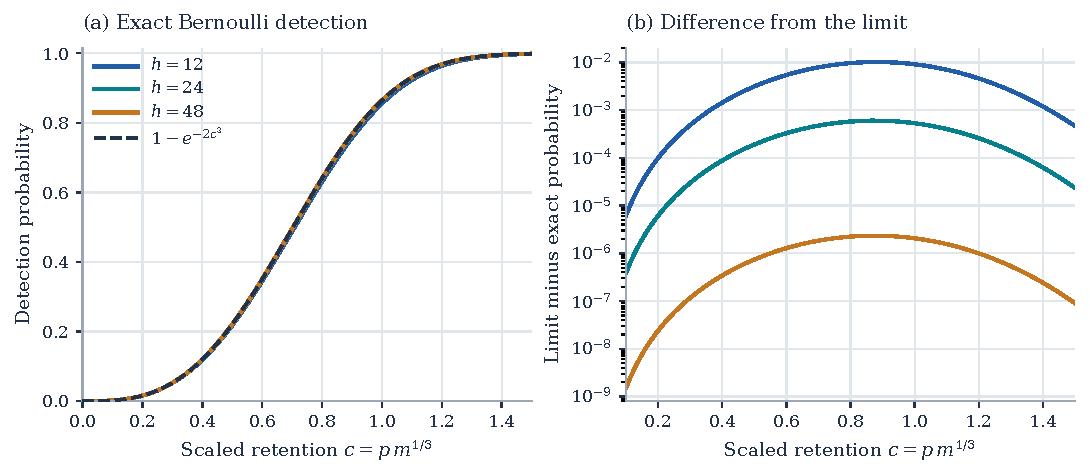
\includegraphics[width=\textwidth]{figures/balanced_sampling.pdf}
\caption{Exact Bernoulli detection probabilities from
\eqref{eq:bernoulli-exact}, with \(p=c m^{-1/3}\), compared with
\(1-e^{-2c^3}\). The right panel resolves the finite-depth deficit
on a logarithmic scale. The finite curves use independent retention;
\cref{thm:main-sampling} proves the same limiting law for fixed-size
uniform samples. The plot evaluates formulas and is not a simulation.}
\label{fig:balanced}
\end{figure}

\section{Optimal sampling by uniform rectangles}
\label{sec:rectangles}

The balanced sampling law does not optimize the number of inspected
entries when the two sample sizes may differ. We now determine that
optimum, including its leading constant, for a single uniformly sampled
rectangle. The sizes \(q_R,q_C\) are fixed before sampling; the row and
column sets are independently uniform among subsets of those sizes.
The entry cost is the deterministic number \(q_Rq_C\).

\subsection{A sparse-row, dense-column limit}

\begin{theorem}[Rectangular detection law]
\label{thm:rectangle-limit}
Fix an anchor size \(s\) for which the preceding construction is pinned.
Suppose, as \(h\to\infty\),
\[
 \frac{q_R}{d_h}\longrightarrow C\in(0,\infty),\qquad
 \frac{q_C}{n}\longrightarrow\theta\in(0,1].
\]
Define
\begin{equation}
 U(C)=1-e^{-C},\qquad w(\theta)=\theta^2(2-\theta).
 \label{eq:rectangle-parameters}
\end{equation}
The probability of observing a complete forbidden copy tends to
\begin{equation}
 F_s(C,\theta)=U(C)
 \left\{1-\left[1-U(C)^s
       \left(1-e^{-Cw(\theta)/2}\right)\right]^2\right\}.
 \label{eq:rectangle-limit}
\end{equation}
In the main construction, \(s=3\) and \(d_h=20h+2\).
\end{theorem}
\begin{proof}
Consider the \(2s\) row anchor groups of the two final minus modes,
the dummy row group, and the two parity halves of the leaf row group.
These disjoint sets have sizes \(m\), except for the last two, which
have size \(m/2\). If their sampled occupancies are \(N_j\) and their
sizes are \(M_j\), then, for fixed nonnegative integers \(\ell_j\),
\begin{equation}
 \E\prod_j\fall{N_j}{\ell_j}
 =\frac{\fall{q_R}{\sum_j\ell_j}}{\fall n{\sum_j\ell_j}}
       \prod_j\fall{M_j}{\ell_j}.
 \label{eq:occupancy-moments}
\end{equation}
Since \(q_R\sim Cd_h\), \(n=d_hm\), and both \(d_h,m\) tend to
infinity, these moments converge to those of independent Poisson
variables: mean \(C\) for every anchor or dummy group and mean \(C/2\)
for each leaf parity group. Tightness, uniform integrability of each
fixed factorial moment, and the multivariate binomial expansion justify
joint convergence exactly as in the proof of \cref{thm:main-sampling}.

The number of sampled leaf rows is tight. The expected number of
sampled sibling pairs is
\[
 \frac m2\frac{\fall{q_R}2}{\fall n2}=O(m^{-1})=o(1).
\]
Thus with probability tending to one these leaves have distinct
parents. For any fixed number of such leaves, their required column
sets---one matching leaf column and two parent-minus columns each---are
disjoint. Under uniform column sampling, the joint inclusion probability
of any \(j\) specified distinct columns is
\(\fall{q_C}j/\fall nj\to\theta^j\). Inclusion-exclusion therefore
gives joint convergence of the inclusion indicators to independent
Bernoulli variables of parameter \(\theta\). Each selected leaf row
receives a successful column mark with probability
\[
 \theta\bigl(1-(1-\theta)^2\bigr)=w(\theta).
\]
The convergence is uniform over the finitely many possible incidence
patterns with a bounded number of leaves. Truncating the tight leaf
count and then removing the truncation proves Poisson thinning: the
successful witness counts in the two parities converge jointly to
independent Poisson variables of mean \(Cw(\theta)/2\), independently
of the limiting row anchor and dummy occupancies.

All \(2s\) relevant column anchor groups are covered with probability
tending to one, since their combined miss probability is at most
\(2s\exp(-q_C/d_h)=o(1)\). In the limit the dummy group is available
with probability \(U(C)\), each parity's row anchors are all available
with probability \(U(C)^s\), and that parity has a witness with
probability \(1-e^{-Cw(\theta)/2}\). The two parity events and the
dummy event are independent. Their combination is
\eqref{eq:rectangle-limit}.
\end{proof}

\subsection{The exact asymptotic entry budget}

For \(z\ge0\), set
\begin{equation}
 \Phi_s(z,\theta)=F_s(z/\theta,\theta)\quad(0<\theta\le1),
 \qquad \Phi_s(z,0)=0,\qquad
 G_s(z)=\max_{0\le\theta\le1}\Phi_s(z,\theta),
 \label{eq:variational-function}
\end{equation}
where \(F_s(0,\theta)=0\) by continuity. The normalization is chosen
so that \(q_Rq_C\sim z d_h^2m\).

\begin{theorem}[Optimal rectangular cost]
\label{thm:optimal-rectangle}
For every \(0<\rho<1\), there is a unique \(z_{\rho,s}>0\) such that
\begin{equation}
 G_s(z_{\rho,s})=\rho.
 \label{eq:optimal-constant}
\end{equation}
Let \(Q_h(\rho)\) be the minimum \(q_Rq_C\) over fixed pairs of
sample sizes whose probability of observing \(H\) is at least \(\rho\).
Then
\begin{equation}
 \lim_{h\to\infty}\frac{Q_h(\rho)}{d_h^2m}=z_{\rho,s}
 =\inf\{C\theta:F_s(C,\theta)\ge\rho,\ C>0,\ 0<\theta\le1\}.
 \label{eq:optimal-rectangle}
\end{equation}
Every maximizing column fraction in \eqref{eq:variational-function},
for \(z>0\), lies strictly between zero and one. Moreover,
\begin{equation}
 z_{\rho,s}>-\log(1-\rho).
 \label{eq:rectangle-lower-constant}
\end{equation}
\end{theorem}
\begin{proof}
The limiting detection probability is bounded by the mean number of
body witnesses, so
\[
 0\le\Phi_s(z,\theta)\le z\theta(2-\theta)\le2z\theta.
\]
This proves continuity at \(\theta=0\), uniformly for bounded \(z\).
Consequently \(G_s\) is continuous. For every fixed \(\theta>0\),
\(\Phi_s(z,\theta)\) is strictly increasing in \(z>0\). A maximizer
for positive \(z\) has \(\theta>0\), so \(G_s\) is also strictly
increasing. It starts at zero, is less than one for every finite \(z\),
and tends to one, as is seen by taking \(\theta=1\). This proves
the existence and uniqueness in \eqref{eq:optimal-constant}, and the
equivalent infimum characterization follows by writing \(z=C\theta\).

For an upper bound on the optimal cost, fix \(z>z_{\rho,s}\) and a
maximizing \(\theta\in(0,1]\). Choose integer sample sizes
\(q_C\sim\theta n\) and \(q_R\sim(z/\theta)d_h\). By
\cref{thm:rectangle-limit}, their detection probability tends to
\(G_s(z)>\rho\), while their normalized cost tends to \(z\).
Letting \(z\downarrow z_{\rho,s}\) proves the required upper bound.

For the lower bound, the upper construction first bounds the optimal
normalized costs. Along a convergent subsequence write
\[
 z_h=\frac{q_Rq_C}{d_h^2m}\longrightarrow z<\infty,
 \qquad \theta_h=\frac{q_C}{n}.
\]
A required leaf diagonal cell gives the finite bound
\begin{equation}
 \Prob(D_{q_R,q_C})\le
 m\frac{q_R}{n}\frac{q_C}{n}=z_h,
 \label{eq:rectangle-finite-lower}
\end{equation}
so \(z\ge\rho>0\). Counting the additional parent column gives the
stronger bound useful for compactness:
\begin{equation}
 \Prob(D_{q_R,q_C})\le
 2m\frac{q_R}{n}\left(\frac{q_C}{n}\right)^2
 =2z_h\theta_h.
 \label{eq:rectangle-compactness}
\end{equation}
Thus \(\theta_h\) stays bounded away from zero. Pass to a further
subsequence with \(\theta_h\to\theta\in(0,1]\). Then
\(q_R/d_h=z_h/\theta_h\to z/\theta\), and
\cref{thm:rectangle-limit} implies \(F_s(z/\theta,\theta)\ge\rho\).
Therefore \(z\ge z_{\rho,s}\), proving the limit.

It remains to locate the optimizer away from the endpoint one.
For fixed \(z>0\), put \(U=1-e^{-z}\), \(v=1-e^{-z/2}\).
Direct differentiation, using
\(Cw(\theta)=z\theta(2-\theta)\), gives
\begin{equation}
 \frac{\partial\Phi_s}{\partial\theta}(z,1)
 =-ze^{-z}U^sv\,[2(s+1)-(2s+1)U^sv]<0.
 \label{eq:interior-optimizer}
\end{equation}
Reducing \(\theta\) slightly from one therefore improves detection
at the same entry cost. Since \(\Phi_s(z,0)=0\), all maximizers
are interior. Finally detection implies a body witness, whose limiting
count is Poisson of mean \(Cw(\theta)\). Hence
\[
 \Phi_s(z,\theta)\le1-e^{-z\theta(2-\theta)}\le1-e^{-z}.
\]
At an interior maximizer the last inequality is strict. Evaluating at
\(z=z_{\rho,s}\) proves \eqref{eq:rectangle-lower-constant}.
\end{proof}

For \(s=3\), numerical optimization gives the illustrative values in
\cref{tab:rectangle-constants}. They approximate the proved variational
constant; the proof does not depend on numerical optimization or on
uniqueness of the maximizing \(\theta\).

\begin{table}[ht]
\centering
\begin{tabular}{ccccc}
\toprule
Target \(\rho\) & \(z_{\rho,3}\) & Optimizing \(\theta\) &
\(C=z/\theta\) & Cost with all columns\\
\midrule
\(1/2\) & 1.314840 & 0.415558 & 3.164034 & 1.852553\\
\(2/3\) & 1.756730 & 0.499090 & 3.519863 & 2.281615\\
\(0.9\) & 2.931197 & 0.647872 & 4.524349 & 3.396702\\
\bottomrule
\end{tabular}
\caption{Numerical values for the five-by-five pattern. The last column
is the solution of \(F_3(C,1)=\rho\); all costs are normalized by
\(d_h^2m\). The supplied script reproduces the calculation.}
\label{tab:rectangle-constants}
\end{table}

\begin{figure}[ht]
\centering
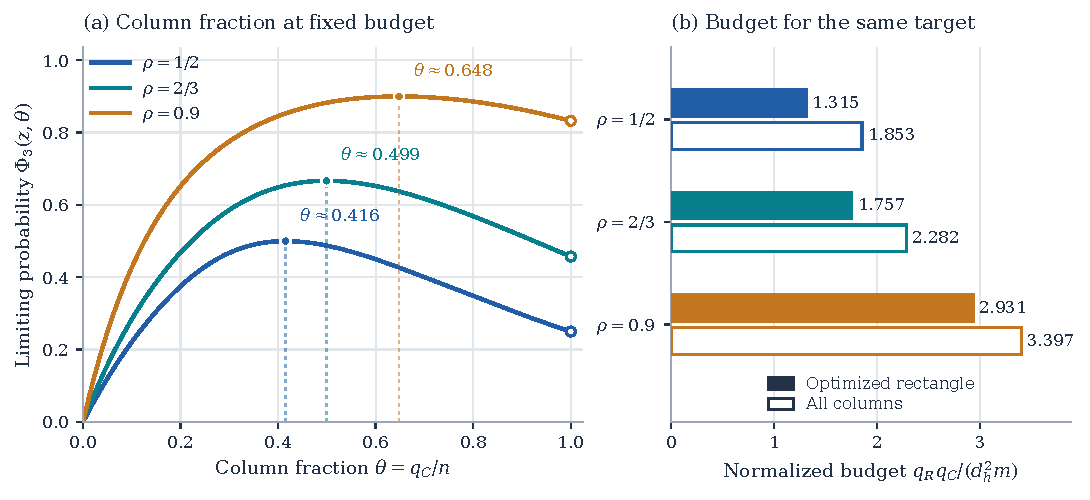
\includegraphics[width=\textwidth]{figures/rectangular_sampling.pdf}
\caption{The limiting detection law at three optimized budgets for
\(s=3\). Filled points mark numerically located maximizers; open
points show all-column sampling at the same budget. No uniqueness
claim is needed. The budget comparison uses the constants of
\cref{tab:rectangle-constants}. The theorem proves the variational
characterization; the plotted locations are numerical approximations.}
\label{fig:rectangular}
\end{figure}

Taking all columns already attains the optimal order
\(\Theta(d_h^2m)\); choosing an interior fraction improves its
constant. Balanced samples instead require
\(\Theta(d_h^2m^{4/3})\) entries at fixed positive detection
probability. The difference is substantial and follows from the
particular three-position witness structure.

\subsection{Scope of the one-sided testing conclusion}

The rows of \(H\) are pairwise distinct, and its columns are pairwise
distinct. This simple fact identifies the strongest possible one-sided
decision rule when the information is one sampled rectangle.

\begin{proposition}[Completion of a negative observation]
\label{prop:completion}
Fix row indices \(r_1<\cdots<r_a\) and column indices
\(c_1<\cdots<c_b\) in \([n]\), where \(a,b\ge1\). Every
\(H\)-free binary matrix \(B\) of size \(a\times b\) extends to
an \(H\)-free \(n\times n\) matrix agreeing with \(B\) at those
prescribed indices. Consequently, among one-sided algorithms observing
only this uniformly sampled rectangle, rejecting whenever a visible
\(H\)-copy occurs is optimal, even when the sampled indices are known.
\end{proposition}
\begin{proof}
Choose nondecreasing surjections \(f:[n]\to[a]\), \(g:[n]\to[b]\)
with \(f(r_i)=i\) and \(g(c_j)=j\); filling the gaps by repeated
neighboring values constructs them. Define
\(\widetilde B(x,y)=B(f(x),g(y))\).
If \(\widetilde B\) contained \(H\), two of its selected rows could
not have the same \(f\)-image: they would have identical traces on
the selected columns, whereas the rows of \(H\) are distinct.
The same holds for selected columns and \(g\). The images are
therefore strictly increasing and give an \(H\)-copy in \(B\), a
contradiction.

An observation with no visible copy is thus consistent with an
\(H\)-free input on precisely the same sampled indices. That sample
has positive probability under the uniform sampling rule. Rejecting
such an observation with positive conditional probability would
violate one-sided correctness on its free completion. The visible-copy
rule rejects every remaining observation and is therefore optimal.
\end{proof}

This proposition and \cref{thm:optimal-rectangle} concern fixed sizes
and one sampled rectangle. They do not determine the optimal query
complexity of arbitrary adaptive entry queries, several sampled
rectangles, or random mixtures of sampling budgets.

\section{Exact inverse logarithmic repair cost}
\label{sec:inversion}

\subsection{The combinatorial relation and its Lambert inverse}

In this section we return to the main pattern: \(s=3\),
\(d=20h+2\), and \(m=2^h\).
Normalize the original-copy transversal by the total number of cells:
\begin{equation}
 \tau_h=\frac{\tau_H(A_h)}{n^2}=\frac{1}{d^2m},\qquad
 \eps_h=\dist_H(A_h)=d^{-2},\qquad a=\frac{\log2}{20}.
 \label{eq:tau-definition}
\end{equation}
Since \(m=\exp(a(d-2))\), the exact relation is
\begin{equation}
 \tau_h=e^{2a}d^{-2}e^{-ad}
       =e^{2a}\eps_h\exp(-a\eps_h^{-1/2}).
 \label{eq:tau-epsilon}
\end{equation}
The total copy density also satisfies the exact identity
\(\delta_h=2\eps_h^3\tau_h^2\).

Let \(W_0\) denote the real principal Lambert function,
characterized on positive arguments by \(W_0(x)e^{W_0(x)}=x\).
\begin{proposition}[Exact inversion]
\label{prop:lambert}
For every \(\tau>0\), the relation
\(\tau=e^{2a}\eps\exp(-a\eps^{-1/2})\) has exactly one positive
solution \(\eps\), namely
\begin{equation}
 \eps(\tau)=
 \frac{a^2}{4W_0\!\left((a/2)e^a\tau^{-1/2}\right)^2}.
 \label{eq:lambert-inverse}
\end{equation}
It agrees with the actual repair distance at \(\tau=\tau_h\).
\end{proposition}
\begin{proof}
Put \(d=\eps^{-1/2}>0\). Taking square roots and rearranging gives
\[
 d e^{ad/2}=e^a\tau^{-1/2},\qquad
 \frac{ad}{2}e^{ad/2}=\frac a2e^a\tau^{-1/2}.
\]
The argument is positive, and \(x\mapsto xe^x\) is strictly
increasing for \(x>0\), proving both the formula and uniqueness.
\end{proof}

This is an application of the existing linear--logarithmic inversion
machinery in ProveIt. The theorem labeled \texttt{p0:thm:lambert-core}
in its transseries manuscript solves \(aX+b\log X=L\) with the
appropriate Lambert branch~\cite{ProveItLambert}. Its positive-parameter
algebraic inversion and uniqueness are also implemented in
\texttt{LinLogCoreInversion.lean}~\cite{ProveItLean}. The present
contribution is the exact combinatorial relation
\eqref{eq:tau-epsilon}, together with its application below and the
explicit convergent coefficient formula. The general Lambert inversion
itself is prior machinery, and no Lean verification of the new matrix
theorems is claimed.

\subsection{A convergent expansion with an explicit remainder}

For sufficiently small \(\tau>0\), define
\begin{equation}
 X=\log(1/\tau)+2\log a+2a,\qquad t=\log X.
 \label{eq:X-inverse}
\end{equation}
Taking logarithms in \eqref{eq:tau-epsilon} shows that
\(u=ad\) is the unique positive solution of
\begin{equation}
 u+2\log u=X.
 \label{eq:inverse-core}
\end{equation}

\begin{theorem}[Convergent logarithmic expansion]
\label{thm:convergent-inverse}
For every real \(X\ge64\), the repair-cost inverse has the absolutely
convergent expansion
\begin{equation}
 \eps(\tau)=\frac{a^2}{X^2}
 \left(1+\sum_{j\ge1}\frac{B_j(\log X)}{X^j}\right),
 \label{eq:convergent-inverse}
\end{equation}
where the rational polynomial \(B_j\) is
\begin{equation}
 B_j(t)=\frac{(-2)^{j+1}}{j!}
 \left.\frac{\dd^{j-1}}{\dd w^{j-1}}
    \frac{(t+\log(1+w))^j}{(1+w)^3}\right|_{w=0}.
 \label{eq:inverse-coefficients}
\end{equation}
It has degree \(j\) and leading coefficient \(2^j(j+1)\). The
first four polynomials are
\begin{align*}
 B_1(t)&=4t,\\
 B_2(t)&=12t^2-8t,\\
 B_3(t)&=32t^3-56t^2+16t,\\
 B_4(t)&=80t^4-\frac{752}{3}t^3+192t^2-32t.
\end{align*}
Put \(r_X=8(\log X+1)/X<1\). For every integer \(N\ge0\),
\begin{equation}
 \left|\eps(\tau)-\frac{a^2}{X^2}
  \left(1+\sum_{j=1}^{N}\frac{B_j(\log X)}{X^j}\right)\right|
 \le\frac{4a^2}{X^2}\frac{r_X^{N+1}}{1-r_X}.
 \label{eq:inverse-remainder}
\end{equation}
\end{theorem}
\begin{proof}
Write \(u=X(1+v)\), \(z=X^{-1}\), and \(t=\log X\). Equation
\eqref{eq:inverse-core} becomes
\begin{equation}
 v=-2z\bigl(t+\log(1+v)\bigr).
 \label{eq:inverse-fixed-point}
\end{equation}
For the moment hold \(t\ge0\) fixed, permit complex \(z\), use the
analytic logarithm on \(|v|<1\), and set \(R_t=1/[8(t+1)]\).
For \(|v|\le1/2\), the power series for the logarithm gives
\( |\log(1+v)|\le\log2<1\). Thus, when \(|z|\le R_t\), the
right side of \eqref{eq:inverse-fixed-point} has modulus at most
\[
 \frac{t+\log2}{4(t+1)}<\frac14,
\]
and its derivative in \(v\) has modulus at most
\(4|z|\le1/[2(t+1)]\le1/2\). Iteration from zero is a uniform
contraction on the closed disk \(|v|\le1/2\). Its analytic iterates
converge locally uniformly to a solution \(v(z,t)\), analytic for
\(|z|<R_t\), with \(|v|\le1/4\).

Apply Lagrange inversion to
\(F(w)=(1+w)^{-2}\) and \(\phi(w)=-2(t+\log(1+w))\):
\[
 [z^j]F(v(z,t))
 =\frac1j[w^{j-1}]F'(w)\phi(w)^j=B_j(t).
\]
For \(t>0\), the coefficient identity follows by changing variable
\(z=w/\phi(w)\) in the coefficient integral and integrating a
derivative; for \(t=0\), it follows by continuity, or directly from
\(v(z,0)=0\). Substituting \(F'\) and \(\phi\) gives
\eqref{eq:inverse-coefficients}. Finite differentiation gives the
displayed first terms. The coefficient of \(t^j\) is obtained from
\((1+w)^{-3}\), since
\[
 \left.\frac{\dd^{j-1}}{\dd w^{j-1}}(1+w)^{-3}\right|_{w=0}
 =(-1)^{j-1}\frac{(j+1)!}{2}.
\]
This yields \(2^j(j+1)\).

On the analytic solution disk, \(|F(v)|\le4\). Cauchy's estimate
on smaller radii and passage to \(R_t\) give
\[
 |B_j(t)|\le4R_t^{-j}=4[8(t+1)]^j.
\]
For \(X\ge64\), one has \(r_X<1\): the function
\(X-8\log X-8\) is increasing for \(X>8\) and positive at
\(64\), using \(\log64=6\log2<6\). Thus \(z=1/X<R_t\),
and the series converges absolutely. The real fixed point satisfies
\(u=X(1+v)>0\). Because \(u+2\log u\) increases from
\(-\infty\) to \(+\infty\), this is the unique solution in
\eqref{eq:inverse-core}. The identity \(\eps=a^2/u^2\) proves
\eqref{eq:convergent-inverse}.

Finally, the coefficient bound gives
\[
 \left|\sum_{j>N}B_j(\log X)X^{-j}\right|
 \le4\sum_{j>N}r_X^j=4\frac{r_X^{N+1}}{1-r_X}.
\]
Multiplication by \(a^2/X^2\) proves the explicit remainder estimate.
\end{proof}

\subsection{A necessary barrier for repair from existing-copy covers}

In particular,
\begin{equation}
 \eps_h\sim\frac{a^2}{\log^2(1/\tau_h)}.
 \label{eq:logarithmic-barrier}
\end{equation}
This is a constraint on any putative universal conversion from the
size of an existing-copy transversal to the size of a successful
binary repair.

\begin{corollary}[Inverse logarithmic obstruction]
\label{cor:inverse-barrier}
Suppose a function \(\Psi:[0,1]\to[0,1]\) satisfies
\[
 \dist_H(A)\le\Psi\!\left(\frac{\tau_H(A)}{n^2}\right)
\]
for every binary \(n\times n\) matrix \(A\). Then
\(\Psi(\tau_h)\ge\eps(\tau_h)\), with the exact inverse and
expansion above. In particular \(\Psi(t)=o(\log^{-2}(1/t))\) as
\(t\downarrow0\) is impossible. If \(\Psi\) is nondecreasing, then
\begin{equation}
 \liminf_{t\downarrow0}\Psi(t)\log^2(1/t)\ge a^2.
 \label{eq:all-t-barrier}
\end{equation}
\end{corollary}
\begin{proof}
Apply the proposed bound to \(A_h\) and use the exact formulas.
For the last assertion, choose \(h\) with
\(\tau_{h+1}\le t\le\tau_h\). Monotonicity gives
\(\Psi(t)\ge\eps_{h+1}\). Also
\[
 \log(1/\tau_{h+1})-\log(1/\tau_h)
 =\log2+2\log\left(\frac{d_h+20}{d_h}\right)=\log2+o(1).
\]
The logarithmic mesh is bounded, so \eqref{eq:logarithmic-barrier}
at \(h+1\) gives \eqref{eq:all-t-barrier}.
\end{proof}

The corollary supplies a necessary lower bound on such a conversion
function. It does not prove a matching universal upper bound for
arbitrary ordered matrices; that remains a separate structural question.

\section{Other branching numbers and the limit of the small anchor}
\label{sec:branching}

\subsection{A family on regular rooted trees}

The full-pattern pinning theorem separates the size of the anchor from
the tree arithmetic. This gives a uniform extension to every fixed
branching number.

\begin{theorem}[Regular branching]
\label{thm:branching}
Fix an integer \(b\ge2\), put \(s=b+1\), and let
\(H^{(b)}=K_{b+1}(P)\) with the body \(P\) in \eqref{eq:H}.
Thus \(H^{(b)}\) has size \((b+3)\times(b+3)\). For every \(h\ge1\),
there is an explicit binary matrix \(A_{b,h}\) with
\begin{equation}
 m=b^h,\quad D_b=2b^2+4b+4,\quad d_h=D_bh+2,\quad n=d_hm,
 \label{eq:bary-size}
\end{equation}
such that
\begin{equation}
 N_{H^{(b)}}(A_{b,h})=b\,m^{2b+4},\qquad
 \dist_{H^{(b)}}(A_{b,h})=d_h^{-2},\qquad
 \tau_{H^{(b)}}(A_{b,h})=\nu_{H^{(b)}}(A_{b,h})=m.
 \label{eq:bary-exact}
\end{equation}
There is an explicit optimal repair of \(m^2\) cells. For independent
uniform balanced samples with \(q/(d_hm^{2/3})\to c\in(0,\infty)\),
the leaf-witness count converges to \(\Poi(bc^3)\), and detection
probability tends to \(1-e^{-bc^3}\).
\end{theorem}
\begin{proof}
Replace the binary tree by the complete \(b\)-ary tree. A block at
depth \(i\) has size \(m/b^i\); nodes are indexed from zero to
\(b^i-1\), and \(\pi(p)=\lfloor p/b\rfloor\). Use the same
recursive orders, placing all \(b\) child subtrees in increasing
order between the two signed blocks. In \eqref{eq:roles}, retain
the two \(V\) modes and use \(W_{i,r}^+,W_{i,r}^-\) for each
residue \(r\in\{0,\ldots,b-1\}\). The same mode order is used
on both axes. Use \(s=b+1\) anchor groups for each mode, with the
same crown and unit-vector signatures. All variable entries are
given by \eqref{eq:entries} with the new parent map.

There are \((2+2b)h\) modes, \(2h+1\) variable classes, and one
dummy class per axis. Their total gives
\[
 d_h=((2+2b)(b+1)+2)h+2=(2b^2+4b+4)h+2.
\]
Every full variable class still has size \(m\). Threshold traces
remain nested, and the anchor signature of a member varies only
with its residue modulo \(b\). Thus there are at most \(b=s-1\)
signatures. The support-pair graph is still two signed paths joined
by the terminal triangle. Its leaf traces remain a chain, now with
\(\lfloor p/b\rfloor\) in place of \(\lfloor p/2\rfloor\).
The crown-exclusion proof, including after the dummy-by-leaf repair,
therefore applies verbatim. Every hypothesis of \cref{thm:pinning}
is verified.

The four order comparisons remain valid with the new parent map.
The body classification uses only those comparisons and the fact
that two child indices in the same residue class have the same
relative order as their parents. It therefore excludes all modes
except \(W_{h,p\bmod b}^-\), where the leaf row and column must
have the same index and the other column belongs to their parent.
That parent block now has \(b\) columns. There are \(m\) leaves,
\(m\) dummy rows, and \(m^{2s}\) anchor choices, giving
\(b m^{2s+2}=b m^{2b+4}\) copies.

The leaf diagonal is an \(m\)-cell transversal. To obtain \(m\)
copies with disjoint row and column sets, assign the \(b\) columns
of each parent bijectively to its children and use distinct dummy
and anchor representatives, as in \cref{thm:packing}. For the edit
lower bound, a uniform leaf chooses its depth-\(i\) ancestor with
probability \(b^{-i}\), so a uniform representative in that node's
block is again uniform on its size-\(m\) class. All protected-cell
probabilities are \(m^{-2}\). The same four propagation bodies
force opposite values at the shared leaf. The explicit repair
\(R_*\times C_h\) excludes every pinned final mode, proving the
matching upper bound.

For the sampling claim, let \(p=q/n\) and let \(X\) count leaves
whose row, matching column, and at least one of their \(b\) parent
columns are sampled. At Bernoulli retention probability \(p\), its
exact generating function is
\begin{equation}
 \E z^X=\left[1-t_b+t_b(1-p^2+p^2z)^b\right]^{m/b},
 \qquad t_b=1-(1-p)^b.
 \label{eq:bary-pgf}
\end{equation}
For fixed-size samples, expand the \(r\)-th factorial moment by
the number \(j\) of distinct parents of its \(r\) leaves.
The distinct-parent tuples number \(m^r(1+O_{b,r}(m^{-1}))\).
Their joint probability is
\(b^r p^{3r}(1+O_{b,r}(p+q^{-1}))\), by inclusion-exclusion on
the disjoint parent blocks. Their contribution tends to
\((bc^3)^r\). Tuples with \(j<r\) parents number \(O_{b,r}(m^j)\)
and have probability \(O_{b,r}(p^{2r+j})\); their contribution is
\(O_{b,r}(m^{-2(r-j)/3})=o(1)\). The earlier factorial-moment
argument gives \(X\Rightarrow\Poi(bc^3)\). All \(b\) final
minus-mode anchors and the dummy row are covered except with
probability at most \((2bs+1)e^{-q/d_h}=o(1)\), proving the
detection limit.
\end{proof}

Put \(a_b=\log b/D_b\). The exact copy density for this family is
\[
 \frac{N_{H^{(b)}}(A_{b,h})}{n^{2b+6}}
 =b\,d_h^{-2b-6}m^{-2}
 =b e^{4a_b}\eps_h^{b+3}
       \exp(-2a_b\eps_h^{-1/2}).
\]
For fixed \(b\), the exponential coefficient is \(2a_b\).

\begin{proposition}[Binary branching optimizes this family]
\label{prop:binary-optimal}
Among integers \(b\ge2\), \(a_b=\log b/(2b^2+4b+4)\) has its
unique maximum at \(b=2\).
\end{proposition}
\begin{proof}
For real \(x\ge2\), the derivative of
\(g(x)=\log x/(2x^2+4x+4)\) has the sign of
\[
 f(x)=2x+4+4/x-(4x+4)\log x.
\]
Its derivative is \(-2-4/x-4/x^2-4\log x<0\), and
\(f(3)=34/3-16\log3<0\). Thus \(g\) decreases on \([3,\infty)\).
The remaining comparison \(g(2)>g(3)\) is equivalent to
\(17\log2>10\log3\), which follows from
\(2^{17}=131072>59049=3^{10}\).
\end{proof}

This optimization concerns the displayed regular-tree family. It does
not constrain constructions using different block weights, variable
branching, different signatures, or another propagation mechanism.

\subsection{Why simply removing another anchor group fails}

The proof of \cref{thm:pinning} uses the body positions essentially;
the three-by-three crown alone is not rigid. Decreasing to two anchor
groups would give the pattern
\begin{equation}
 H_4=\begin{pmatrix}
 0&1&1&0\\1&0&0&1\\1&0&1&0\\0&1&1&1
 \end{pmatrix}.
 \label{eq:H4}
\end{equation}
The same host and repair no longer work.

\begin{proposition}[A four-by-four copy surviving the proposed repair]
\label{prop:H4-counterexample}
Form the binary host at depth \(h=2\) using \(s=2\) anchor groups.
Both this host and its dummy-by-leaf repair contain an unpinned copy
of \(H_4\).
\end{proposition}
\begin{proof}
Select, in order, the following four rows:
\[
 \widehat R_{V_2^+}(2),\quad
 \widehat R_{W_{2,0}^-}(2),\quad R_2(2),\quad R_*.
\]
One arbitrary representative is chosen from each displayed block.
Select columns from
\[
 \widehat C_{W_{2,0}^-}(1),\quad
 C_1^+(0),\quad C_1^+(1),\quad C_1^-(1).
\]
The mode order gives the row order, and the recursive column order
gives the stated column order. The first two rows have traces
\(0110\) and \(1001\) by their anchor incidences. For leaf index
\(2\), the parent index is \(1\), so its trace is \(1010\).
The dummy row has trace \(0111\). These are exactly the rows of
\(H_4\). There are no selected leaf columns, so the repair changes
none of these entries. Only one selected column is an anchor,
exhibiting the failure of full-pattern pinning.
\end{proof}

This is a counterexample to this particular two-group construction
and repair argument. It neither proves polynomial removal for every
four-by-four pattern nor excludes a different four-by-four obstruction.

\section{Research questions suggested by the exact construction}
\label{sec:questions}

The preceding theorems settle concrete refinements of the reviewed
source construction. The following questions identify further work;
none is used as an assumption in the proofs.

\begin{question}[Small forbidden matrices]
What is the least \(k\) for which a binary \(k\times k\) pattern
fails polynomial ordered removal? The present work gives \(k\le5\).
Determine which patterns of orders two, three, and four admit
polynomial removal. In particular, can one control the additional
\(H_4\)-copies in \cref{prop:H4-counterexample} by a different repair
and counting argument, or find a different small anchor-body pattern?
\end{question}

\begin{question}[The strength of the removal obstruction]
For the explicit \(H\) in \eqref{eq:H}, determine the asymptotic
order of \(\mathcal R_H(\eps)\). Can the construction be improved
to give \(\mathcal R_H(\eps)\le\exp(-c\eps^{-\alpha})\) with
\(\alpha>1/2\), or can a matching lower bound of stretched-exponential
type be proved? Reducing the number of protected classes, allowing
unequal block sizes, or sharing anchors across levels are concrete
directions. \Cref{prop:binary-optimal} rules out an improvement of
the exponential coefficient from changing only the regular branching
number in the displayed family.
\end{question}

\begin{question}[Universal repair from a transversal]
Define
\[
 \Gamma_H(t)=\sup\left\{\dist_H(A):
         \tau_H(A)/n^2\le t,\quad A\in\{0,1\}^{n\times n},\ n\ge1\right\}.
\]
Does \(\Gamma_H(t)=O(\log^{-2}(1/t))\) hold for the five-by-five
pattern, or can the gap between original-copy covering and binary
repair be larger? The construction proves
\(\liminf_{t\downarrow0}\Gamma_H(t)\log^2(1/t)\ge a^2\).
A matching upper bound would turn the inverse logarithmic obstruction
into a sharp structural theorem for all hosts.
\end{question}

\begin{question}[Structure and stability of optimal repairs]
Classify all \(m^2\)-cell repairs of \(A_h\). More generally, what
must an \(H\)-free matrix differing in at most \((1+\eta)m^2\)
cells look like as \(\eta\downarrow0\)? Is there a finite collection
of repair mechanisms near which every near-minimizer lies, or do
many distributed repairs attain the same cost? Exact distance alone
does not resolve the geometry of the minimizing edits.
\end{question}

\begin{question}[A quantitative Poisson approximation]
Obtain explicit total-variation error bounds for the fixed-size
witness law, uniformly when \(q/(d_hm^{2/3})\) ranges in a compact
subset of \((0,\infty)\). Separate the correction to the mean,
sibling dependence, and sampling without replacement. Determine the
first finite-depth correction to the detection quantile, including
the error from anchor coverage. The exact factorial moments and
Bernoulli generating function provide independent starting points.
\end{question}

\begin{question}[Uniqueness and asymptotics of the optimal rectangle]
Is \(\theta\mapsto\Phi_s(z,\theta)\) unimodal for every \(s\ge3\)
and \(z>0\)? Determine the optimizer and \(z_{\rho,s}\) as
\(\rho\downarrow0\), \(\rho\uparrow1\), or \(s\to\infty\).
The interior-optimizer theorem does not imply uniqueness. It would
also be useful to determine whether randomized sample budgets or
several rectangles improve expected entry cost at a fixed detection
probability.
\end{question}

\begin{question}[Adaptive information]
What lower bounds survive when a tester may choose arbitrary entries
adaptively? A fixed explicit host has copies at known locations, so
uniform-sampling lower bounds alone cannot answer this. Construct
distributions of ordered hosts that hide the relevant modes and leaf
witnesses while preserving distance, and analyze one-sided and
two-sided adaptive testers separately. The extension argument in
\cref{prop:completion} suggests a precise information-completion
criterion for partial observations beyond rectangles.
\end{question}

\begin{question}[Other witness exponents]
Can related ordered constructions force a critical witness to use
\(r\) rare sampled positions, for fixed \(r>3\), while retaining
an exact repair theorem and a fixed forbidden pattern? With \(m\)
potential witnesses, the heuristic scale would become
\(q\asymp d_hm^{1-1/r}\). A proof must control overlapping witnesses
and anchor coverage; the heuristic by itself supplies neither.
\end{question}

\begin{question}[General full-pattern pinning]
Replace the crown and the two unit-vector signatures in
\cref{thm:pinning} by other fixed binary patterns. Which combinatorial
conditions on nested classes, signature counts, and the body force
the prefix to lie in a single anchor mode? A classification could
separate the part of an anchor that is rigid by itself from the
additional rigidity supplied by the body, and provide smaller
obstructions in other ordered induced-removal problems.
\end{question}

\section{Source record, verification, and integration}
\label{sec:verification}

\subsection{What was reviewed and what is proved here}

The source review is fixed to the following repository snapshots,
retrieved on 7 October 2026:
\begin{itemize}
\item \texttt{openai/math}, commit\\
\texttt{adc7f1241b42e322a6451854ab7e4b4c146bf78a}.
The selected item is Family 190, \emph{Polynomial removal fails for
ordered binary matrices}, manuscript date 25 September 2026.
The construction, original anchor argument, distance proof, counting
argument, conclusion, and bibliography were read. Its formalization
catalogue identifies a Lean comparator for the \(66\times66\)
nonpolynomial-removal theorem~\cite{OAI190Lean}; that upstream project
was not rebuilt during this work.
\item \texttt{VladimirReshetnikov/ProveIt}, commit\\
\texttt{fb9602e556560a15704b4feb176ba6de08378665}.
The relevant sources are the transseries theorem
\texttt{p0:thm:lambert-core} and the file
\texttt{LinLogCoreInversion.lean}. The exact positive-parameter
inversion and uniqueness statements were checked at the source level.
Those existing Lean modules were not rebuilt here.
\end{itemize}

OpenAI's repository explicitly distinguishes results at different
stages of verification~\cite{OAIRepo}. ProveIt's repository similarly
distinguishes formal theorems, executable certificates, and exploratory
research material~\cite{ProveIt}. These distinctions motivate the
choice of a finite combinatorial construction whose essential steps
can be written out and tested independently. This article is a focused
research extension, not a certification of all results in either
repository.

The inherited ingredients are the signed-tree host, its role table and
orders, its nonanchor threshold entries, and its protected-path
propagation lower bound. The new refinements established here are the
full-pattern pinning theorem and five-by-five obstruction; the repair
that attains the lower bound and the proof that it creates no copies;
the exact classification, count, packing, and transversal; the finite
sampling identities and sharp limits; the optimal uniform-rectangle
cost; the exact transversal-to-repair relation with its explicit
convergent logarithmic expansion; and the stated regular-tree
generalization. The standard Lambert inversion is credited separately.
Novelty is asserted relative to the reviewed source results; no claim
of a global minimum pattern size or an exhaustive priority search is
made.

\subsection{Reproducible finite and numerical checks}

The companion program \texttt{code/verify.py} uses only Python's
standard library, exact integers, and rational arithmetic. It implements
the construction independently of the written pinning proof. Equal
rows or columns inside a block are represented by one weighted
position. Since every row and every column of \(H\) is distinct,
an \(H\)-copy cannot choose two positions from one such twin block;
weighted compressed enumeration therefore counts the expanded host
exactly.

The default checks include the following:
\begin{itemize}
\item Exhaustive searches for complete \(H\)-copies at depths one and
two, in both the original and repaired hosts. The compressed orders
are \(23\) and \(47\); the search examines all \(33{,}649\) and
\(1{,}533{,}939\) row five-tuples, respectively, and all compatible
column chains. Every original copy has its full prefix pinned.
The exact expanded counts are \(512=2\cdot2^8\) and
\(131{,}072=2\cdot4^8\); both repaired counts are zero.
\item Structural nesting, signature, and nonanchor crown checks through
depth six; explicit disjoint expanded copies; and weighted body
enumeration in every designated mode. Completeness of the latter
enumeration for arbitrary depth is justified by the written pinning
theorem, not inferred from testing.
\item An explicit \(H_4\)-copy surviving repair, as in
\cref{prop:H4-counterexample}, and small-host checks of the failure
of crown-only pinning.
\item Exact Bernoulli formulas checked by enumerating all relevant
leaf-row, leaf-column, and parent-column outcomes in small instances.
The independent anchor and dummy events are integrated analytically.
\item The fixed-size factorial-moment identity checked against every
row and column sample in witness submodels \((m,n)=(2,6),(4,10)\),
for all \(q\in\{0,\ldots,n\}\) and every order \(1\le r\le m\):
\(58\) exact rational comparisons in total.
\end{itemize}

The output \texttt{code/verification\_results.json} records the
parameters and outcomes. The checks use explicit exceptions, so they
also run under Python's optimization flag. They check the repair's
size and small-depth freeness; they do not search all possible edit
sets or computationally prove the general \(m^2\) lower bound.

The optional script \texttt{code/verify\_inversion.py} checks the
first logarithmic coefficient polynomials symbolically when SymPy is
installed, and evaluates
the exact inverse and remainder estimates at high precision.
\texttt{code/generate\_figures.py} reproduces the vector figures and
the illustrative rectangular constants using NumPy, SciPy, and
Matplotlib. Its probabilities are evaluations of exact formulas;
the numerical optimizers are approximations, not certified interval
enclosures. The analytic theorems do not rely on those optimizations.

\subsection{A concrete route to formalization}

The finite structural core offers a natural first integration target
for ProveIt. A staged dependency order is preferable to treating
the whole article as one formalization obligation:
\begin{enumerate}
\item Define ordered binary copies by increasing embeddings and prove
the twin-block compression lemma and the completion lemma.
\item Formalize \cref{thm:pinning} as an abstract finite theorem.
Its proof uses order, distinct traces, set inclusion, and a bounded
number of signatures; it does not require probability or limits.
\item Define the signed tree positions and entries, then prove the
four order comparisons, the signature bound, and nonanchor crown
exclusion for the original and repaired hosts.
\item Prove copy classification, exact count, the explicit packing,
and repair freeness. These give finite identities for every \(h\).
\item Formalize the arbitrary-edit lower bound by counting protected
selections, or by finite probability. The shared-path dependence
must remain explicit; the proof only uses independence for protected
cells, not for arbitrary variable pairs.
\item Add finite sampling identities. Poisson convergence and
rectangular asymptotics can follow as separate analytic modules.
For the inverse, reuse ProveIt's existing principal Lambert core
and formalize the specialized combinatorial substitution and the
analytic contraction remainder.
\end{enumerate}

The archive supplies the article, complete LaTeX build inputs, exact
verification code, numerical scripts, and their receipts. It introduces
no new axiom declarations or unproved Lean stubs. The new theorems are
presented as mathematical proofs with supplementary checks, ready for
independent review and subsequent formalization.

\bibliographystyle{plain}
\begingroup\raggedright
\bibliography{references}
\endgroup
\end{document}
